%%%%%%%%%%%%%%%%%%%%%%%%%%%%%%%%%%%%%%%%%
% Structured General Purpose Assignment
% LaTeX Template
%
% This template has been downloaded from:
% http://www.latextemplates.com
%
% Original author:
% Ted Pavlic (http://www.tedpavlic.com)
%
% Note:
% The \lipsum[#] commands throughout this template generate dummy text
% to fill the template out. These commands should all be removed when 
% writing assignment content.
%
%%%%%%%%%%%%%%%%%%%%%%%%%%%%%%%%%%%%%%%%%

\documentclass{article}

\usepackage{fancyhdr} % Required for custom headers
\usepackage{lastpage} % Required to determine the last page for the footer
\usepackage{extramarks} % Required for headers and footers
\usepackage{graphicx} % Required to insert images
\usepackage[latin1]{inputenc}

% Margins
\topmargin=-0.45in
\evensidemargin=0in
\oddsidemargin=0in
\textwidth=6.5in
\textheight=9.0in
\headsep=0.25in 

\linespread{1.1} % Line spacing



\setlength\parindent{0pt} % Removes all indentation from paragraphs

%----------------------------------------------------------------------------------------
%	DOCUMENT STRUCTURE COMMANDS
%	Skip this unless you know what you're doing
%----------------------------------------------------------------------------------------

% Header and footer for when a page split occurs within a problem environment
\newcommand{\enterProblemHeader}[1]{
\nobreak\extramarks{#1}{#1 continued on next page\ldots}\nobreak
\nobreak\extramarks{#1 (continued)}{#1 continued on next page\ldots}\nobreak
}

% Header and footer for when a page split occurs between problem environments
\newcommand{\exitProblemHeader}[1]{
\nobreak\extramarks{#1 (continued)}{#1 continued on next page\ldots}\nobreak
\nobreak\extramarks{#1}{}\nobreak
}

\setcounter{secnumdepth}{0} % Removes default section numbers
\newcounter{homeworkProblemCounter} % Creates a counter to keep track of the number of problems
%----------------------------------------------------------------------------------------
%	NAME AND CLASS SECTION
%----------------------------------------------------------------------------------------

\newcommand{\lessonNumber}[1]{Lezione\ \##1} % Assignment title
\newcommand{\lessonDate}[4]{#1,\ #2\ #3\ #4} % Due date
\newcommand{\lessonCourse}[1]{#1} % Course/class
\newcommand{\lessonTime}[1]{#1} % Class/lecture time
\newcommand{\lessonTeacher}[1]{#1} % Teacher/lecturer
\newcommand{\lessonAuthor}[1]{#1} % Your name
\begin{document}
\section{Lezione 2}
% Mercoledì 2 Ottobre 2013

La tecnologia evolve ad una velocità incontrollabile, diventa obsoleta rapidamente. Bisogna capire la differenza tra le cose \textbf{essenziali} e le cose \textbf{accidentali}. Tra le cose essenziali c'è la disciplina, tra le cose accidentali ci sono la tecnica e gli strumenti, E' importante concentrarsi sugli aspetti fondamentali e non accidentali. Occorre avere capacità di impegno concettuale, di astrazione, di analisi e rigore (\textit{best practice}). Vogliamo utilizzare la traccia di chi ha fatto le cose in passato e le ha \textbf{fatte bene}. Queste cose sono irraggiungibili senza impegno.

\textbf{Progetto didattico}: ci sono due approcci alternativi ed uno spazio intermedio. Bisogna fornire competenze per affrontare \textit{challenges} (sfide) sempre più alte. Il metodo di insegnamento deve portare a trovare il punto di ottimo.

\begin{center}

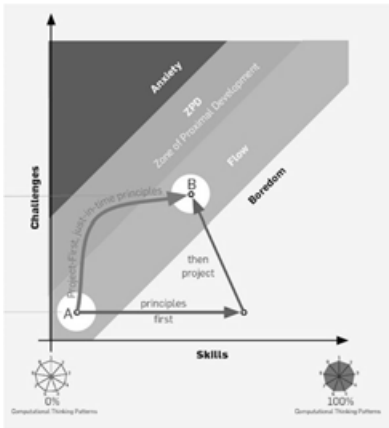
\includegraphics[width=0.75\columnwidth]{img1} % Example image

\end{center}

Nello spazio bianco c'è la \textbf{noia sicura}. Il principio opposto è la \textbf{sfida immediata}, in cui bisogna fare leva sui principi. C'è una cosa da fare e questa cosa è \textbf{ambiziosa}.

\textbf{Cosa non è un progetto}: mettere un accrocchio di cose che sembrano funzionali (progetti fatti finora), non è il ``\textit{basta che respiri}'', è opporre il principio di \textbf{by correction} a quello di \textbf{by construction} (costruire sapendo che funzionerà). In questo modo si fa fatica subito ma meno in seguito. Niente correzioni in fase di sviluppo.

Cosa è un progetto:

\begin{itemize}

	\item \textbf{Pianificazione}: pianifica chi sa cosa vuole fare, è l'essenza per controllarsi, per sapere se stiamo convergendo o divergendo. Ogni attività inizia con la \textbf{pianificazione};
	\item \textbf{Analisi dei requisiti}: si analizza ciò di cui si ha bisogno. L'analisi ha un'importanza decisiva, bisogna capire il problema;
	\item \textbf{Progettazione}: si decide la forma della soluzione. Solo dopo si passa alla:
	\item \textbf{Realizzazione}: dove sta anche la programmazione, che deve aderire al 100\% alla progettazione. Nella realizzazione attuo, ma non sono ancora sicuro che il risultato soddisfi il cliente, ergo:
	\item \textbf{Verifica e validazione};
	\item \textbf{Manutenzione}: per la maggior parte della sua vita il prodotto resta in manutenzione. Non esiste vita operativa senza manutenzione, non esiste software perfetto, quindi esso dev'essere mantenuto costantemente;
	\item \textbf{Qualità}: uno dei principi su cui punteremo, perchè la qualità è possibile. Vorremmo quantificare la qualità in modo oggettivo.

\end{itemize}

\textbf{Libri}: ``\textit{Fare imparando}''. I libri aiutano poco e servono solo come appoggio o approfondimento. I concetti vanno vissuti nel progetto.

\textbf{Libri teorici}, servono solo nel piano delle skills.

\textbf{Libri esperienziali}, ``\textit{si fa così perchè l'ho fatto}''.

È importante costruire il proprio \textbf{glossario}.

\textbf{SWEBOK} (swe body of knowledge): non è un libro per apprendere ma per risolvere dubbi; strutturato in 10 aree di conoscenza. L'essenza dell'esame sarà il progetto didattico da svolgere da metà Novembre fino alla fine dell'anno. Progetto di gruppo di minimo 6 e massimo 7 persone. ~100 ore di studio individuale.

\textbf{Attività di gruppo}: attività ripartite con rotazione dei ruoli. Ciò non terrà conto delle abilità, nessuno è essenziale: è un danno all'efficienza ma è un beneficio didattico. Nessuno fa cose in autonomia, dev'essere tutto deciso secondo un piano \textbf{regolato}. Nessuno fa in modo estroso, ma disciplinato e sistematico.

\textbf{Analisi del problema da risolvere}, concentrarsi sulle cose essenziali e trovare una soluzione buona per costruzione.

\textbf{Approccio ingegneristico}, disciplinato, sistematico, quantificabile.

\textbf{Proccessi software}, attività coordinate, processi di ciclo di vita per far evolvere il sw da uno stato all'altro. Il sw è una macchina a stati:

\begin{itemize}

	\item \textbf{Concezione};
	\item \textbf{Sviluppo};
	\item \textbf{Utilizzo};
	\item \textbf{Ritiro}.

\end{itemize}

Nella fase di ritiro il software cessa di esistere nel senso che non c'è più alcun tipo di supporto per quel prodotto. Le transizioni sono strettamente e formalmente regolate.

\textbf{Modelli di ciclo di vita}

\textbf{Iterazione ed incremento}: iterazione significa che faccio una cosa più volte finchè non raggiungo un limite; incremento significa aggiungere, è additivo. Sono incrementale solo se aggiungo, è un obiettivo molto importante da raggiungere (e potenzialmente distruttivo, potrebbe far perdere tempo). Iterare significa riprovare, non ripetere. Non si può togliere quando si è incrementali.

\textbf{Prototipo}, serve per imparare, è tipicamente “usa e getta”. Viene diviso in due categorie: quelli rivolti al cliente, per fargli capire cosa avrà, e quelli rivolti verso di noi per aiutarci a trovare una soluzione. Quelli rivolti verso di noi sono un costo, mentre quelli rivolti verso il cliente sono un valore aggiunto. Il primo impatto tra l'utente e il prodotto è l'\textbf{interfaccia}. I prototipi possono essere ``usa e getta'' ma costano tempo.

\textbf{Riuso}: il sw che già esiste è la maggior parte del nostro prodotto. L'informatico deve insegnare a \textit{riusare} in modo sistematico e non opportunistico. Il riuso è cosa saggia se so approvvigionarmi da un fornitore intelligente.

La manutenzione richiede gestione della storia, \textbf{versionamento}. Bisogna avere una storia del proprio prodotto. Bisogna spiegare e documentare la scelta ed avere una tecnica che salvi la storia (\textbf{repository}).

\begin{center}

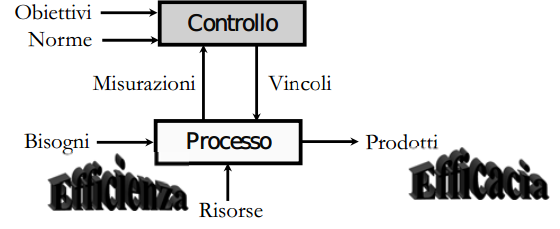
\includegraphics[width=0.75\columnwidth]{img2} % Example image

\end{center}

L'efficienza si vede dove vedo il consumo di risorse. L'efficacia si misura guardando i prodotti e vedendo se sono buoni o cattivi rispetto alla produzione. Un processo è un insieme di attività coordinate e coese (tutti hanno bisogno di tutti).

Standard di riferimento: ISO/IEC 12207.

\end{document}
